\documentclass[tikz, border=10pt]{standalone}

% Required packages for drawing, positioning, shapes, arrows, and colors
\usepackage{tikz}
\usepackage{xcolor}
\usetikzlibrary{
    positioning,      % For placing nodes relative to each other (e.g., right=of)
    shapes.geometric, % For shapes like 'rounded rectangle'
    arrows.meta,      % For modern arrow tips like 'Stealth'
    shadings          % To create gradient fills
}

% Define custom colors based on the image for easy reuse and modification
% Border color for the blocks
\definecolor{BorderColor}{HTML}{424A7F}
% Gradient start color (left side of the blocks)
\definecolor{LeftGradient}{HTML}{E4DFFF}
% Gradient end color (right side of the blocks)
\definecolor{RightGradient}{HTML}{D9F3FF}

\begin{document}

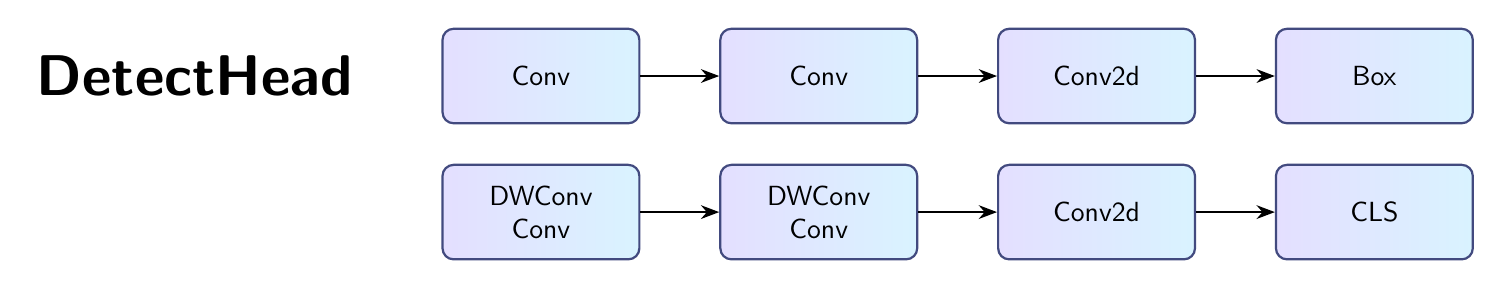
\begin{tikzpicture}[
    % Set global node distance: 0.5cm vertical, 1cm horizontal
    node distance=0.5cm and 1cm,
    % Set the default font to sans-serif to match the image
    font=\sffamily,
]
    % --- Define TikZ styles for diagram elements ---

    % Style for the main blocks (nodes)
    \tikzset{
        block/.style={
            shape=rectangle,         % Use a rectangle with rounded corners
            rounded corners=4pt,   % Adjust the radius of the corners
            draw=BorderColor,                % Set the border color
            thick,                           % Make the border line thick
            shade,                           % Apply a gradient fill
            left color=LeftGradient,         % Gradient starting color
            right color=RightGradient,       % Gradient ending color
            align=center,                    % Center-align text (for multi-line nodes)
            minimum height=1.2cm,            % Set a minimum height for consistency
            minimum width=2.5cm,             % Set a minimum width for consistency
        },
        % Style for the arrows connecting the blocks
        arrow/.style={
            draw,                            % This is a drawable element
            thick,                           % Make the arrow line thick
            -Stealth                         % Use the 'Stealth' arrowhead from arrows.meta
        }
    }

    % --- Place the diagram elements ---

    % 1. Place the main title node on the left
    % The font is set to be large, bold, and sans-serif
    \node[font=\sffamily\bfseries\huge] (title) {DetectHead};

    % 2. Place the top row of blocks
    % The first block is placed 2cm to the right of the title
    \node[block, right=1cm of title] (conv1) {Conv};
    % Subsequent blocks are placed to the right of the previous one
    \node[block, right=of conv1]     (conv2) {Conv};
    \node[block, right=of conv2]     (conv2d1) {Conv2d};
    \node[block, right=of conv2d1]   (box) {Box};

    % 3. Place the bottom row of blocks
    % The first block is placed below the first block of the top row
    \node[block, below=of conv1]     (dwconv1) {DWConv\\Conv};
    % Subsequent blocks are placed to the right of the previous one
    \node[block, right=of dwconv1]    (dwconv2) {DWConv\\Conv};
    \node[block, right=of dwconv2]    (conv2d2) {Conv2d};
    \node[block, right=of conv2d2]    (cls) {CLS};

    % 4. Draw the arrows connecting the blocks
    % Top row arrows
    \draw[arrow] (conv1.east) -- (conv2.west);
    \draw[arrow] (conv2.east) -- (conv2d1.west);
    \draw[arrow] (conv2d1.east) -- (box.west);

    % Bottom row arrows
    \draw[arrow] (dwconv1.east) -- (dwconv2.west);
    \draw[arrow] (dwconv2.east) -- (conv2d2.west);
    \draw[arrow] (conv2d2.east) -- (cls.west);

\end{tikzpicture}

\end{document}